% Placeholder for numbers that are filled in once the benchmark is frozen.
\providecommand{\tbd}{\textbf{[TBD]}}
\providecommand{\figplaceholder}[1]{\fbox{\parbox[c][0.28\linewidth][c]{0.96\linewidth}{\centering\small Figure placeholder: #1}}}

\section{Empirical evaluation}\label{sec:experiments}
We evaluate \method as a causal amortized Bayesian filter on two simulated systems and two robot datasets, and compare it with three particle-filter baselines that learn their transition and measurement models from the same data. All four datasets are observed through the same heavy-tailed, multimodal measurement noise, so that the comparison also tests how each method copes with a non-Gaussian likelihood. We evaluate the accuracy of the filtering distributions, the calibration of their uncertainty intervals, the sensitivity to the noise model, and the inference cost. All methods have the same information access, use the same data splits and update budgets, and are scored with the same metrics. Every number in this section is produced from the frozen run directories by the scripts listed in Appendix~\ref{app:reproducibility}.

\subsection{Datasets}\label{sec:experiments-data}
Table~\ref{tab:datasets} summarizes the four datasets. Each sequence consists of a known initial state, a control sequence, and noisy observations of the subsequent states. The reference states are used only for training and scoring. Every dataset is split by trajectory or episode before windowing, and normalization statistics are computed on the training split only.

\paragraph{Observation noise.}
Each observed coordinate is corrupted independently by the same three-component Gaussian mixture,
\begin{equation}\label{eq:obsnoise}
 V\sim 0.70\,\N\!\big(0,(0.5\sigma)^2\big)+0.15\,\N\!\big(2.5\sigma,(1.5\sigma)^2\big)+0.15\,\N\!\big(-2.5\sigma,(1.5\sigma)^2\big),
\end{equation}
whose scale $\sigma$ is 0.1 for the pendulum (in rad and rad/s), 0.5 for Lorenz--96, and 0.1 in normalized units for the two robot datasets. The mixture has standard deviation $1.65\,\sigma$. The Gaussian with the same mean and variance has total-variation distance 0.332 to this mixture and this number is a reference point for Section~\ref{sec:experiments-noise}.

\begin{table}[t]
\centering\footnotesize
\begin{tabular}{lllll}
\toprule
 & Pendulum & Lorenz--96 & ALOHA insertion & REASSEMBLE \\
\midrule
Source & simulated & simulated & sim.\ demonstrations & real robot \\
State dimension $d$ & 2 & 12 & 14 & 7 \\
Observed coordinates & 2 & 6 & 14 & 7 \\
Control dimension & 1 & -- & 14 & 9 \\
Observation noise & mixture, $\sigma=0.1$ & mixture, $\sigma=0.5$ & mixture, $\sigma=0.1$ & mixture, $\sigma=0.1$ \\
Time step $\Delta t$ & 0.05 & 0.02 & 0.02 & 1/30 \\
Window length (steps) & 60 & 100 & 250 & 250 \\
Train / val.\ / test windows & 224 / 48 / 48 & 1600 / 200 / 100 & 400 / 50 / 50 & 2000 / 300 / 300 \\
Samples / particles $M$ & 128 & 200 & 200 & 500 \\
Metric units & physical & physical & normalized & normalized \\
\bottomrule
\end{tabular}
\caption{Datasets. The observation noise is the mixture of Equation~\eqref{eq:obsnoise} with the stated scale $\sigma$; ``sim.\ demonstrations'' refers to human teleoperation recorded in simulation. $M$ is the number of posterior draws scored per window (Appendix~\ref{app:protocol}).}
\label{tab:datasets}
\end{table}

\paragraph{Controlled pendulum.}
A damped pendulum driven by a scalar torque $u$, simulated as the It\^o SDE
\begin{equation}\label{eq:pendulum}
 d\theta=\omega\,dt+\sigma_\theta\,dW_\theta,\qquad
 d\omega=\Big(\frac{u}{m\ell^{2}}-c\,\omega-\frac{g}{\ell}\sin\theta\Big)dt+\sigma_\omega\,dW_\omega,
\end{equation}
with $g=9.81$, $\ell=m=1$, damping $c=0.2$, and process-noise scales $\sigma_\theta=0.01$ and $\sigma_\omega=0.2$, integrated by Euler--Maruyama with eight substeps per observation interval $\Delta t=0.05$. The initial state is known to every filter and drawn as $\theta_0\sim\mathrm{U}(-\pi,\pi)$, $\omega_0\sim\N(0,0.6^{2})$. Both coordinates are observed. 

\paragraph{Lorenz--96.}
The twelve-dimensional Lorenz--96 system,
\begin{equation}\label{eq:lorenz96}
 \frac{dx_i}{dt}=(x_{i+1}-x_{i-2})x_{i-1}-x_i+F,
 \qquad i=0,\ldots,11,\qquad F=8,
\end{equation}
with cyclic indices, integrated with a fourth-order Runge--Kutta scheme at $\Delta t=0.02$. Each window is an independent trajectory: its initial state is drawn as $x(0)\sim\N(0,\,0.01^{2}I)$, integrated for a spin-up of 500 steps so that it lies on the attractor, and the state at the end of the spin-up is the known initial state $x_0$ of the window. Only every second coordinate is observed, so six coordinates must be inferred from the dynamics alone. 

\paragraph{ALOHA insertion.}
Bimanual peg-insertion demonstrations from the ALOHA simulation benchmark, recorded by human teleoperation at 50\,Hz \citep{zhao2023aloha}. Each frame stores two different 14-dimensional joint vectors, which we keep apart: the \emph{commanded} joint positions (the leader-arm targets sent to the position controllers of the follower arms) serve as the control input, and the \emph{measured} joint positions of the follower arms define the state. The two differ by the tracking error of the controllers, which is largest during contact. The recorded states are deterministic given the commands, so we perturb them by a slowly varying latent disturbance (a four-dimensional AR(1) velocity offset whose magnitude grows with the tracking error, that is, during contact) before normalization. The exact recipe is given in Appendix~\ref{app:reproducibility}. The perturbed trajectory is the reference state, and it is observed through the noise of Equation~\eqref{eq:obsnoise} with $\sigma=0.1$ in normalized units. 

\paragraph{REASSEMBLE.}
Contact-rich assembly and disassembly episodes recorded on a real seven-degree-of-freedom robot arm at 30\,Hz \citep{sliwowski2025reassemble}. The state consists of the seven joint positions and all states are obesrvable. The nine-dimensional robot commands serve as controls. Unlike the other datasets, the dynamics are those of a physical system interacting with its environment, and no model of them is available.

\subsection{Compared Methods}\label{sec:experiments-methods}
All four methods are causal Bayesian filters: the estimate of $x_{k+1}$ uses the observations up to and including $y_{k+1}$, starts from the known initial state. NF-DPF, NSF, and FlowSDE are used in particle filters, which obtain their uncertainty from the observations through Bayesian weighting with learned transition and measurement models. NF-DPF also learns an observation-conditioned proposal, whereas NSF and FlowSDE run as bootstrap filters. \method infers the state distribution directly from the observations. For the two simulated systems, pendulum and Lorenz--96, we also report model-based reference filters that use the true dynamics and the true noise scale: an extended Kalman filter (EKF) and an unscented Kalman filter (UKF) with the moment-matched Gaussian likelihood, and a bootstrap particle filter with the exact mixture likelihood. These references indicate the accuracy attainable with perfect models and are not competitors.

\subsection{Benchmark Results}\label{sec:experiments-results}
Table~\ref{tab:main-results} compares the four methods on four datasets. Each configuration is trained with three independent seeds, and we report the mean and standard deviation over seeds. Accuracy is measured by the RMSE of the posterior mean, averaged over test windows. Distributional accuracy is measured by the continuous ranked probability score (CRPS) and the energy score \citep{gneiting2007proper}, averaged over coordinates. Calibration is measured by the empirical coverage of central 90\% marginal intervals, pooled over windows, steps and coordinates, which is read together with their mean width. Inference cost is the median wall-clock time to filter one test window on a single GPU.

\begin{table}[htbp]
\centering\footnotesize
\resizebox{\linewidth}{!}{%
\begin{tabular}{llccccc}
\toprule
Dataset & Method & RMSE $\downarrow$ & CRPS $\downarrow$ & Cov.\ 90\% & Width & Latency (ms) $\downarrow$ \\
\midrule
Pendulum & \method & 0.0691 $\pm$ 0.0008 & 0.0362 $\pm$ 0.0004 & 0.834 $\pm$ 0.017 & 0.1862 $\pm$ 0.0093 & \textbf{6.7} \\
 & NF-DPF & \textbf{0.0629 $\pm$ 0.0007} & \textbf{0.0320 $\pm$ 0.0003} & \textbf{0.918 $\pm$ 0.006} & 0.2017 $\pm$ 0.0017 & 14.5 \\
 & NSF & 0.0687 $\pm$ 0.0029 & 0.0346 $\pm$ 0.0014 & 0.866 $\pm$ 0.035 & 0.1805 $\pm$ 0.0110 & 12.6 \\
 & FlowSDE & 0.1144 $\pm$ 0.0069 & 0.0578 $\pm$ 0.0026 & 0.918 $\pm$ 0.003 & 0.3107 $\pm$ 0.0012 & 16.2 \\
 & EKF / UKF & 0.0578 $\pm$ 0.0000 & 0.0296 $\pm$ 0.0000 & 0.870 $\pm$ 0.001 & 0.1650 $\pm$ 0.0002 & 12.3 / 12.2 \\
 & bootstrap PF & 0.0406 $\pm$ 0.0003 & 0.0192 $\pm$ 0.0001 & 0.895 $\pm$ 0.002 & 0.1129 $\pm$ 0.0000 & 10.4 \\
\midrule
Lorenz--96 & \method & 0.2942 $\pm$ 0.0082 & 0.1586 $\pm$ 0.0040 & 0.880 $\pm$ 0.016 & 0.8715 $\pm$ 0.0394 & \textbf{14.2} \\
 & NF-DPF & 0.2899 $\pm$ 0.0086 & 0.1585 $\pm$ 0.0051 & 0.854 $\pm$ 0.022 & 0.7811 $\pm$ 0.0645 & 30.9 \\
 & NSF & \textbf{0.2290 $\pm$ 0.0173} & \textbf{0.1199 $\pm$ 0.0103} & 0.822 $\pm$ 0.019 & 0.4692 $\pm$ 0.0053 & 20.6 \\
 & FlowSDE & 0.3227 $\pm$ 0.0067 & 0.1749 $\pm$ 0.0043 & \textbf{0.890 $\pm$ 0.009} & 0.9554 $\pm$ 0.0412 & 33.4 \\
 & EKF / UKF & 0.0229 $\pm$ 0.0000 & 0.0093 $\pm$ 0.0000 & 0.997 $\pm$ 0.000 & 0.0906 $\pm$ 0.0001 & 12.7 / 19.0 \\
 & bootstrap PF & 0.0188 $\pm$ 0.0001 & 0.0077 $\pm$ 0.0000 & 0.990 $\pm$ 0.000 & 0.0674 $\pm$ 0.0000 & 15.4 \\
\midrule
ALOHA & \method & \textbf{0.0538 $\pm$ 0.0011} & \textbf{0.0301 $\pm$ 0.0007} & \textbf{0.871 $\pm$ 0.013} & 0.1645 $\pm$ 0.0017 & \textbf{19.5} \\
 & NF-DPF & 0.1307 $\pm$ 0.0288 & 0.0780 $\pm$ 0.0186 & 0.658 $\pm$ 0.065 & 0.2278 $\pm$ 0.0031 & 49.7 \\
 & NSF & 0.0858 $\pm$ 0.0006 & 0.0501 $\pm$ 0.0004 & 0.821 $\pm$ 0.005 & 0.2339 $\pm$ 0.0012 & 37.8 \\
 & FlowSDE & 0.0717 $\pm$ 0.0004 & 0.0413 $\pm$ 0.0002 & 0.858 $\pm$ 0.006 & 0.2147 $\pm$ 0.0047 & 49.4 \\
\midrule
REASSEMBLE & \method & \textbf{0.0326 $\pm$ 0.0016} & \textbf{0.0179 $\pm$ 0.0008} & \textbf{0.903 $\pm$ 0.005} & 0.1026 $\pm$ 0.0022 & \textbf{21.4} \\
 & NF-DPF & 0.0613 $\pm$ 0.0006 & 0.0340 $\pm$ 0.0003 & 0.858 $\pm$ 0.004 & 0.1760 $\pm$ 0.0021 & 47.8 \\
 & NSF & 0.0615 $\pm$ 0.0002 & 0.0345 $\pm$ 0.0001 & 0.916 $\pm$ 0.000 & 0.2140 $\pm$ 0.0003 & 43.0 \\
 & FlowSDE & 0.0530 $\pm$ 0.0012 & 0.0300 $\pm$ 0.0007 & 0.951 $\pm$ 0.001 & 0.2136 $\pm$ 0.0045 & 57.3 \\
\bottomrule
\end{tabular}
}
\caption{Test results, mean $\pm$ standard deviation over three training seeds, with $M$ posterior draws per window as in Table~\ref{tab:datasets} and, for the particle filters, the particle count of the dataset protocol (500, 1000, 200, 500). RMSE and width are in the metric units of Table~\ref{tab:datasets}. Coverage is nominally 0.90. Latency is the median time in milliseconds to filter one test window in the configuration of the row (seed 0, one NVIDIA L40S, compilation excluded). For the EKF / UKF, latency is measured with the same protocol.}
\label{tab:main-results}
\end{table}

\paragraph{Robot datasets.}
On ALOHA and REASSEMBLE, \method attains the lowest RMSE and CRPS by a wide margin, with the narrowest intervals and a coverage close to the nominal level (0.87 and 0.90). Here the transition dynamics are high-dimensional, and for REASSEMBLE they are those of a physical, contact-rich system. The particle filters rely on a learned one-step transition model and a learned measurement density, and errors in either directly affect their weights. NF-DPF in particular loses accuracy and coverage on ALOHA. \method instead learns the observation-conditioned update directly and uses every observed coordinate without an explicit likelihood.

\paragraph{Simulated systems.}
On the pendulum and Lorenz--96, particle filters with learned models are more accurate than \method: NF-DPF reaches the lowest RMSE on the pendulum and NSF on Lorenz--96. Both systems have smooth, low-dimensional dynamics that a one-step transition model can learn accurately from clean state pairs, and once these models are accurate, Bayesian weighting is close to optimal. The reference filters put the numbers in perspective. On the pendulum, the exact-likelihood particle filter with the true model reaches 0.041, whereas the Gaussian filters with the true dynamics but the moment-matched likelihood (EKF, UKF) reach only 0.058 and a coverage of 0.87: three quarters of the gap between the best learned filter and the model-based filters is caused by the noise model alone, a point we return to in Section~\ref{sec:experiments-noise}. On Lorenz--96 the reference particle filter reaches 0.019, an order of magnitude below every learned method, but it owes this to the exact chaotic dynamics. The learned methods, at 0.23 to 0.32, therefore operate at the accuracy of a dynamics model with a few percent error, which the chaotic flow amplifies over the window, and the six unobserved coordinates can only be inferred through that model. NSF, the most accurate learned method on Lorenz--96 but at a much more under-covered level (0.82).

\paragraph{Calibration.}
Figure~\ref{fig:calibration} shows the empirical coverage of central intervals at nominal levels from 10\% to 95\%. \method lies on the diagonal on Lorenz--96, ALOHA and REASSEMBLE at every level (within 0.03, 0.04 and 0.05 of the nominal level, respectively), so its intervals are calibrated as a whole and not only at 90\%. On the pendulum it is under-dispersed at every level by about one tenth (0.45 at the 50\% level, 0.83 at 90\%). The shortfall is concentrated in the angle coordinate during the first steps after the known initial state, where the predictive spread grows more slowly than the error (angle coverage 0.80 against 0.87 for the velocity, and 0.62 over the first five steps). The particle filters are miscalibrated in both directions depending on the dataset: NF-DPF is over-dispersed on the pendulum (0.56 at the 50\% level) and strongly under-dispersed on ALOHA (0.33 at 50\%, 0.66 at 90\%). FlowSDE is over-dispersed on the pendulum and REASSEMBLE (0.63 at 50\%). NSF is under-dispersed at the high levels on Lorenz--96 and ALOHA (0.82 at 90\%). At equal accuracy \method's intervals are also the narrowest (Table~\ref{tab:main-results}: 0.16 against 0.21--0.23 on ALOHA, 0.10 against 0.18--0.21 on REASSEMBLE). The reference filters are over-dispersed on Lorenz--96 (coverage 0.99 at the 90\% level with the validation-selected process noise), so even the true model does not yield calibrated intervals on the chaotic system.

\begin{figure}[htbp]
\centering
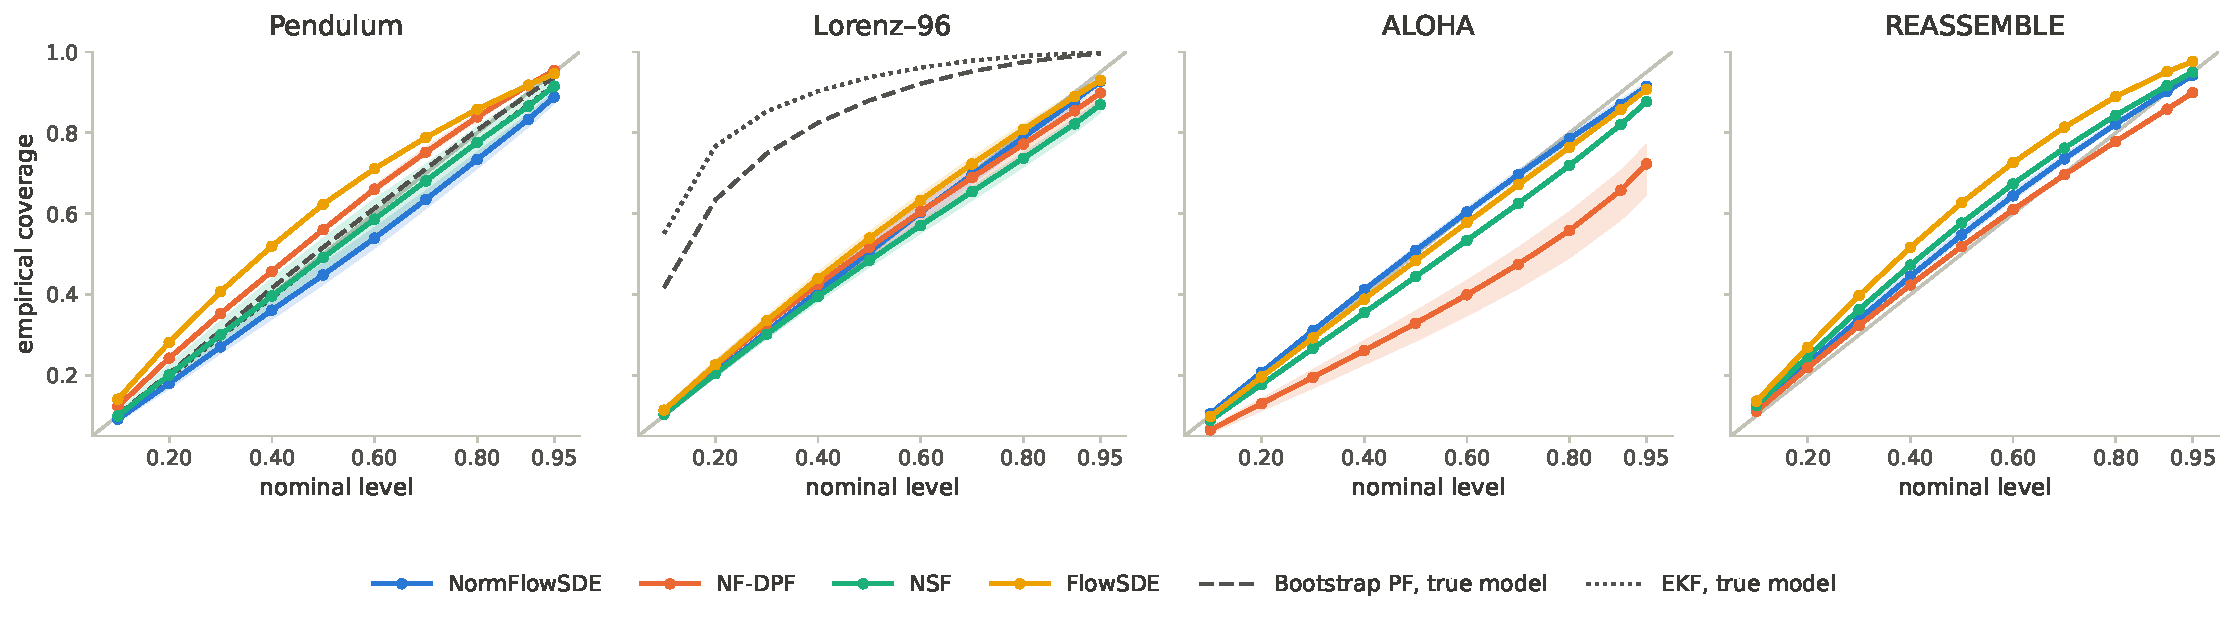
\includegraphics[width=\linewidth]{figures/calibration.pdf}
\caption{Calibration of central marginal intervals at nominal levels from 10\% to 95\%, pooled over test windows, steps, and coordinates (mean over three seeds; shaded: range over seeds). The diagonal indicates perfect calibration. Gray curves: reference filters with the true model on the simulated systems.}
\label{fig:calibration}
\end{figure}

\paragraph{Latency.}
A \method sample requires one network evaluation per time step, without weighting or resampling. A particle filter additionally evaluates the measurement density for every particle at every step and resamples when the effective sample size drops. The latency column of Table~\ref{tab:main-results} reports the median time to filter one test window in the configuration of each row. \method is the fastest method on every dataset, by a factor of 1.5 to 2.0 over the fastest particle filter and 2.3 to 2.7 over the slowest. The advantage is largest on the two robot datasets, where the 14- and 7-dimensional measurement densities are the most expensive part of the particle filters.

\subsection{Observation-Noise Recovery}\label{sec:experiments-noise}
The mixture noise of Equation~\eqref{eq:obsnoise} is the main difference between this benchmark and the usual Gaussian setting. The reference filters in Table~\ref{tab:main-results} already show its price for a method with the wrong noise model: with the true dynamics, the Gaussian filters lose a third of their accuracy on the pendulum relative to the exact-likelihood particle filter (0.058 against 0.041). We therefore investigate wether the learned method actually recover the noise distribution from data.

\begin{figure}[t]
\centering
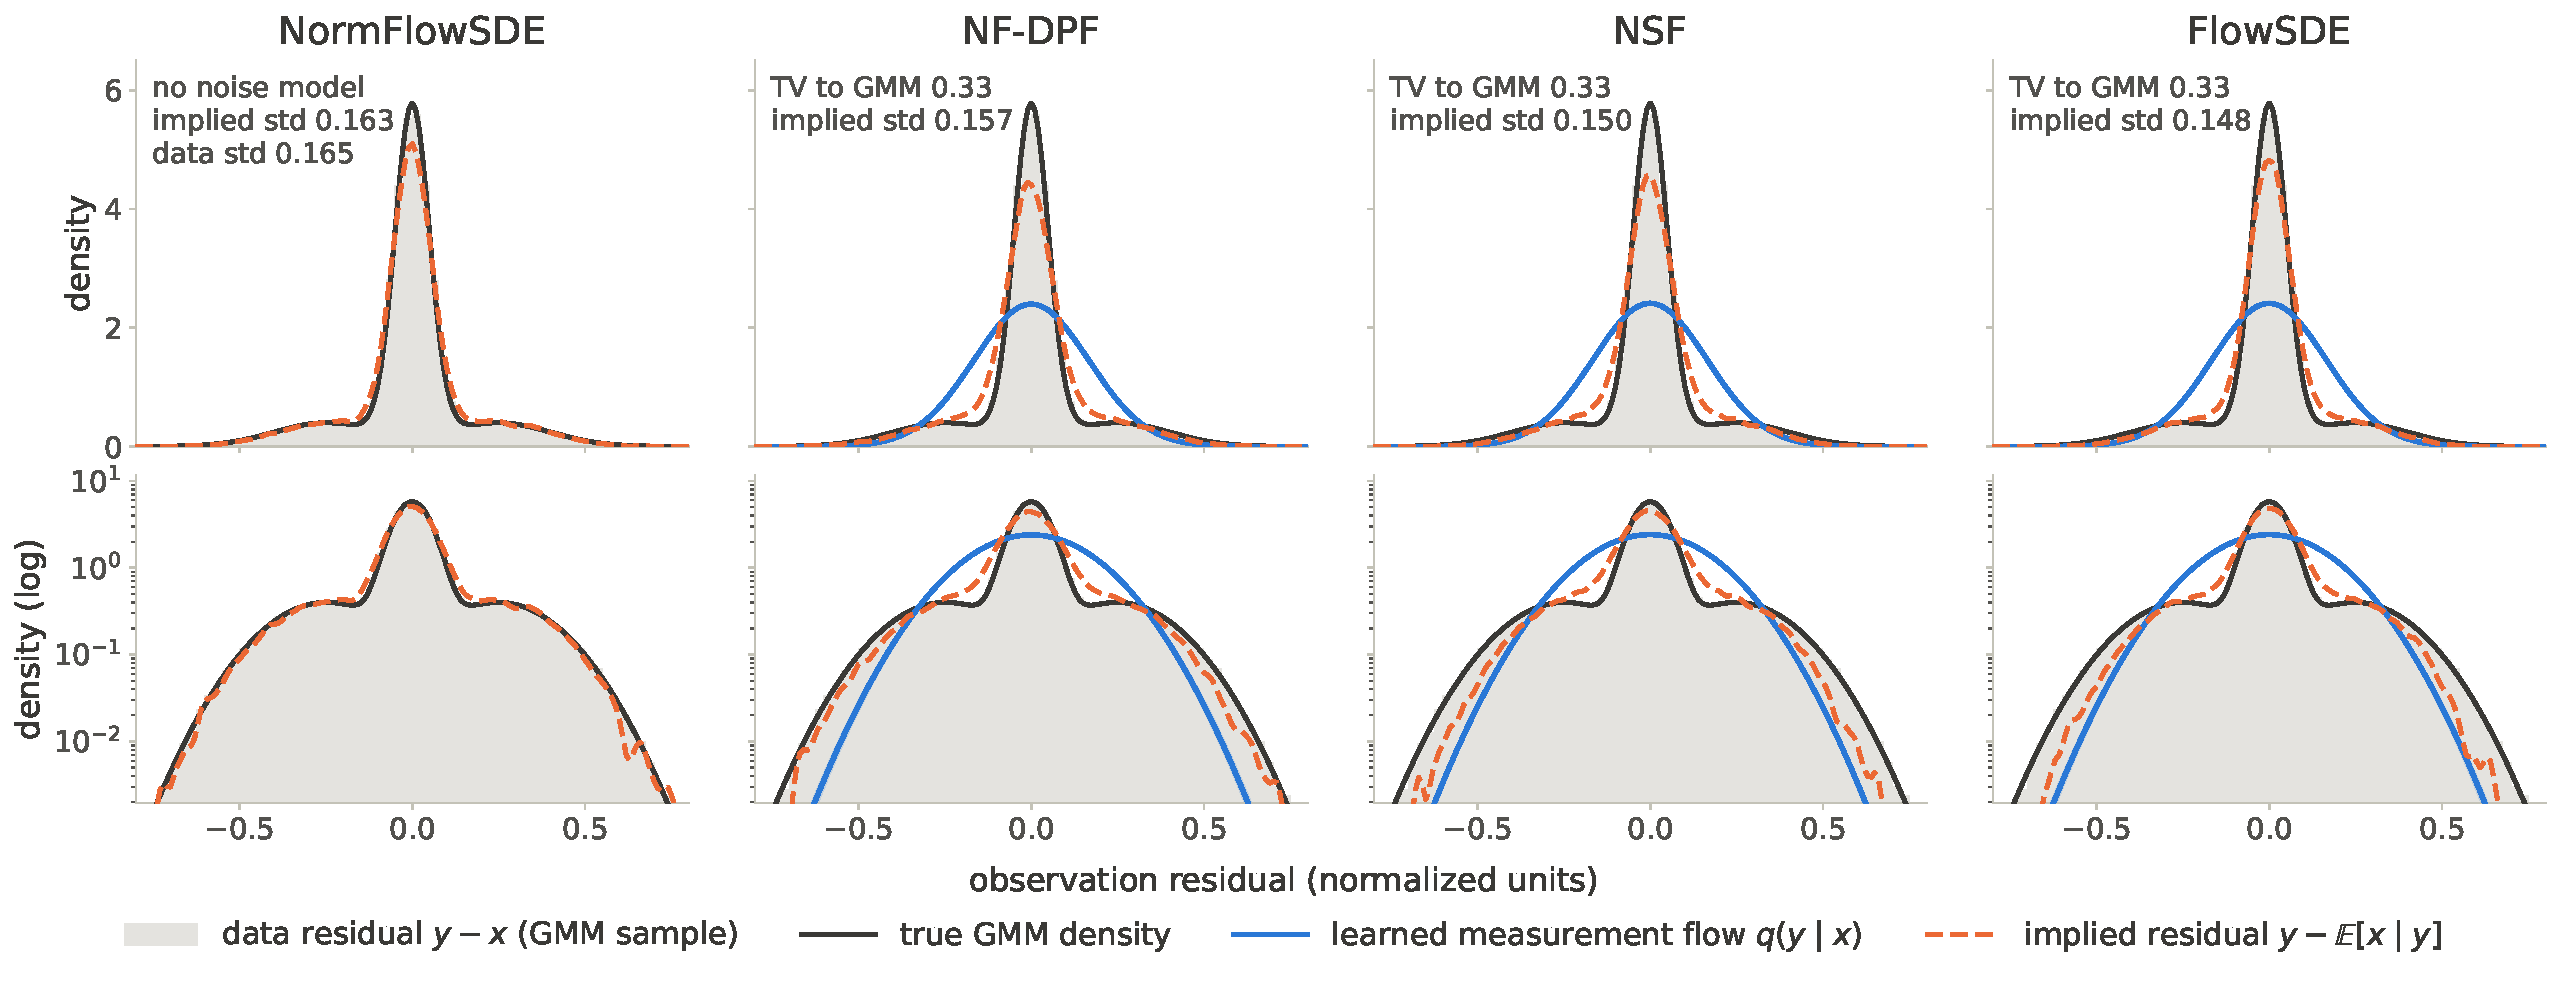
\includegraphics[width=\linewidth]{figures/measurement_density_reassemble.pdf}
\caption{Recovery of the observation noise on REASSEMBLE (seed 0, normalized units). Gray: histogram of the data residuals $y-x$; black: the mixture of Equation~\eqref{eq:obsnoise}; blue: the learned measurement flow $q(y\mid x)$ of each particle filter, averaged over 100 test states and all coordinates (band: 10th to 90th percentile over states); orange, dashed: the implied residuals $y-\E[x\mid y]$ of each method's posterior mean. Top: linear scale; bottom: logarithmic scale. The three learned flows coincide with the moment-matched Gaussian (total variation 0.33 to the mixture, analytic value 0.332), whereas the implied residuals of \method follow the mixture.}
\label{fig:noise-recovery}
\end{figure}

Figure~\ref{fig:noise-recovery} compares the learned measurement densities with the true mixture on REASSEMBLE. For the three particle filters we evaluate the learned conditional flow $q(y\mid x)$ along one-coordinate slices $y=x+\delta e_j$ around test states and average over states and coordinates. \method has no measurement model. For every method we show the distribution of the implied residuals $y-\E[x\mid y]$, which means the observations minus the posterior mean. The result is the same for all three particle filters: the learned measurement flows match the variance of the noise but none of its shape. Their total-variation distance to the mixture is 0.33, which equals the analytic distance (0.332) between the mixture and its moment-matched Gaussian. This indicates the flows have converged to the moment-matched Gaussian. 

Three consequences follow. (i) The learned particle filters weight their particles with a Gaussian likelihood on mixture data: too little weight on particles that agree with a measurement from the sharp central component, too little tolerance for the side modes. They therefore inherit the deficit of the EKF and UKF in Table~\ref{tab:main-results}. (ii) Three flows with different architectures and training signals stop at the same density on every dataset. A conditional affine coupling flow on a Gaussian base, fitted by maximum likelihood, has little incentive to move beyond the second moment when the heavy tails appear in only a few percent of the training pairs. (iii) \method recovers the noise structure implicitly. Its implied residuals reproduce the mixture over four decades of density on every dataset, including central spike and side modes with a standard deviation within 4\% of the data. Trained on the rollout objective alone, the amortized update has learned how much to trust each measurement: one from the sharp central component is highly informative, whereas one from a side mode is much less so. This is exactly the information that a correct likelihood encodes. The implied residuals of the particle filters are sharper than their learned likelihoods, because resampling with the dynamics partly corrects the wrong weights. But the residual spread of NSF and FlowSDE is 7\% to 10\% below the data: their posterior means follow the noisy measurements rather than the state.

\subsection{Summary}\label{sec:experiments-summary}
\method is the most accurate filter on both robot datasets, is calibrated at all nominal levels on three of the four datasets, and is the fastest method on every dataset. On the two simulated systems, particle filters with accurately learned dynamics are more accurate. This advantage stems from their importance weighting. However, the noise-recovery analysis shows the price of that weighting: the learned measurement densities of all three particle filters collapse to the moment-matched Gaussian, so they weight their particles with the wrong likelihood, whereas the amortized update of \method reproduces the mixture implicitly. \method is therefore most attractive when the dynamics are complex or physical and hard to model explicitly, when the measurement noise is not Gaussian, and when fast and calibrated inference is required.
